% !TeX spellcheck = es_ANY
% Chapter 1

%\chapter{Chapter Title Here} % Main chapter title
%
%\label{Chapter1} % For referencing the chapter elsewhere, use \ref{Chapter1} 

%----------------------------------------------------------------------------------------

% Define some commands to keep the formatting separated from the content 
\newcommand{\keyword}[1]{\textit{#1}}
%\newcommand{\tabhead}[1]{\textbf{#1}}
%\newcommand{\code}[1]{\texttt{#1}}
%\newcommand{\file}[1]{\texttt{\bfseries#1}}
%\newcommand{\option}[1]{\texttt{\itshape#1}}

%----------------------------------------------------------------------------------------

\chapter{Introducción}
	La termodinámica es el estudio de las transformaciones de energía. En la etapa más temprana de esta rama de las ciencias, se pensaba que el calor era una clase de fluido cuya cantidad neta en el universo permanecía siempre constante. El aumento de temperatura de un cuerpo era explicado a partir de la migración de calor de un objeto a otro \cite{feynman2011feynman, fermi1986}. Usando dicha teoría del calor como fluido, el ingeniero Sadi Carnot dio origen a la termodinámica con el análisis del problema, sobre cómo generar el mejor y más eficiente motor de vapor en 1824. Posteriormente, Julius von Mayer en 1842 descubrió una equivalencia entre el calor y el trabajo mecánico, relaci\'on también publicada por James Joule el siguiente año \cite{fermi1986}. A raíz de esto hoy se considera el calor como una forma de transferencia de energía \cite{fermi1986}.
	
	Los resultados de la termodinámica se encuentran implícitos en una serie de declaraciones que reciben el nombre de leyes de la termodinámica, las cuales, en conjunto, nos permiten conocer la dirección natural en la que tienen lugar los cambios químicos y físicos en la materia \cite{atkins2011physical}. Históricamente la termodinámica fue desarrollada antes que se tuviera un entendimiento sobre la estructura interna de la materia, además, sus leyes tampoco siguen un orden cronológico \cite{feynman2011feynman}. La primera ley surge del trabajo realizado por Mayer en 1842, una de las leyes más importantes de la ciencia en general: la conservación de la energía \cite{feynman2011feynman, fermi1986}. La segunda, se atribuye a Carnot y Clausius en 1824, y habla sobre la reversibilidad o direccionalidad de los procesos \cite{feynman2011feynman}.
	
	A pesar que el estudio de las transformaciones de energía parece un tema distante de la química, la termodinámica, estudiada a través de la fisicoquímica, ha demostrado ser de vital importancia tanto en la química como la biología \cite{atkins2011physical}. No sólo permite entender la producción o consumo de energía en las reacciones químicas, sino que, constituye una herramienta fundamental para responder preguntas que se encuentran en el corazón de la bioquímica, por ejemplo sobre cómo fluye la energía en una célula, y qué tan grande puede ser la agrupación de moléculas que forman estructuras complejas como las células \cite{atkins2011physical}. En otros casos, por ejemplo, existen propiedades de fácil determinación para un analista, como el color, masa y densidad. Sin embargo, hay propiedades que dependen de los enlaces, estructura molecular y naturaleza del material, entre estas se encuentran propiedades termodinámicas de interés químico, como lo son: la capacidad calorífica, entalpía, entropía, etc \cite{gaisford2016principles}.
	
	Dentro de la fisicoquímica, el estudio y medición de la transferencia de energía en forma de calor se denomina calorimetría, y constituye una de las áreas más antiguas de esta rama de la química \cite{zielenkiewicz2006theory}. Se podría considerar que la historia de esta comienza en junio de 1783, con la presentación de \textit{Memoria del calor} (Mémoire de la Chaleur) por Lavoisier y Laplace en la Academia Francesa \cite{zielenkiewicz2006theory}. La mayoría de los procesos físicos y químicos están acompañados de absorción o liberación de energía. Lo anterior hace de la calorimetría una técnica con un amplio rango de aplicaciones \cite{wadso2001standards}. Entre estas aplicaciones se encuentran titulaciones, flujos, reacciones y estudio de procesos de adsorción \cite{gaisford2016principles}.
		
	El instrumento para realizar estas mediciones se denomina calorímetro, y los hay de diversos tipos. Pueden ser clasificados por el tipo de condiciones que imponen al sistema, por ejemplo, volumen constante, temperatura constante, calor constante, etc. Estos calorímetros reciben el nombre de: bombas calorimétricas, isotérmicos, y adiabáticos, respectivamente \cite{gaisford2016principles, wadso2001standards}. También pueden ser clasificados por el principio de funcionamiento, si compensan los flujos de energía o los acumulan \cite{gaisford2016principles}. Finalmente, dependiendo del rango de las potencias medidas, se tienen dos términos comúnmente usados: \keyword{microcalorimetría} para el caso de experimentos realizados en el rango de los microvatios \cite{wadso2001standards, wadso2003new}, mientras que para escalas de nanovatios son usados \keyword{nanocalorímetros} \cite{wadso2003new}.
	
	En particular, el trabajo que se expone en el presente documento, instal\'o, y calibr\'o un microcalorímetro 2277 Thermal Activity Monitor. Para esto fue necesario el entendimiento del funcionamiento del calorímetro a nivel interno, desde las partes hidra\'ulicas, pasando por los detalles de la electrónica hasta los principios fisicoquímicos detrás del mismo. Para confirmar que el calor\'imetro se encontraba operando de forma correcta se realizaron m\'ultiples calibraciones el\'ectricas, tanto est\'aticas como din\'amicas, las cuales resultan ser un proceso rutinario en la operaci\'on del calor\'imetro. Este calor\'imetro en particular funciona mediante el principio de transferencia de energ\'ia, en donde la diferencia de energ\'ia producida al interior de una celda de medici\'on ,fluye a trav\'es de dos elementos Peltier en un esfuerzo por establecer el equilibrio t\'ermico con los alrededores, lo cual se muestra en la \autoref{fig: heatFlow} \cite{Suurkuusk}.
	\begin{figure}[h]
		\centering
		\begin{subfigure}{0.59\linewidth}
			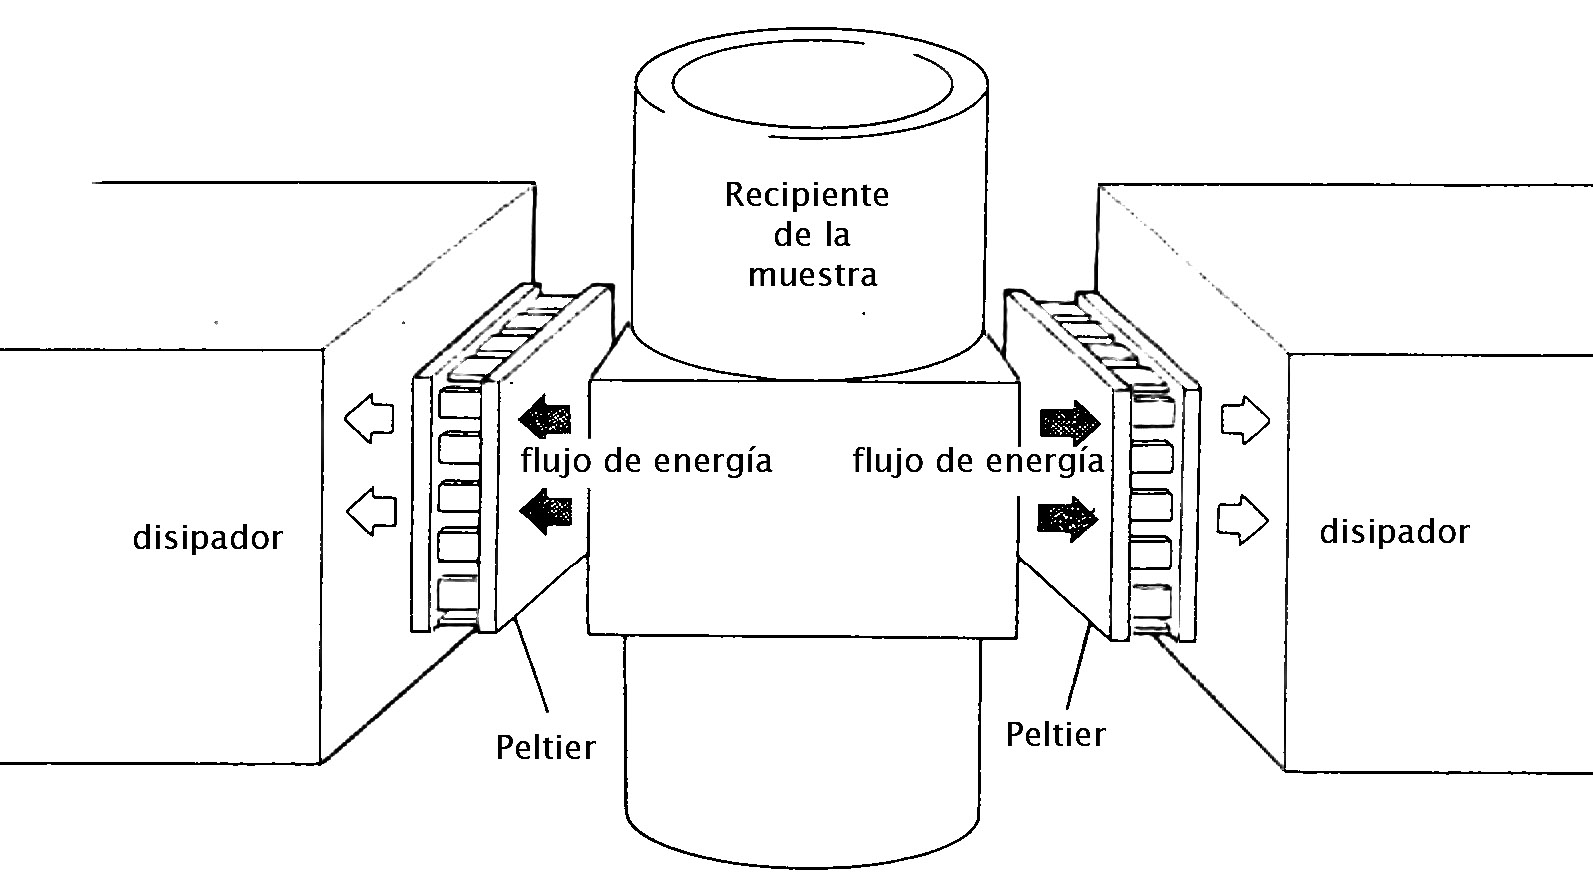
\includegraphics[width=\linewidth]{Figures/heatFlow}
			\caption{Interacci\'on de la celda de medici\'on con los alrededores, modificado de \cite{Suurkuusk}.}
			\label{fig: heatFlow}
		\end{subfigure}
		\begin{subfigure}{0.39\linewidth}
			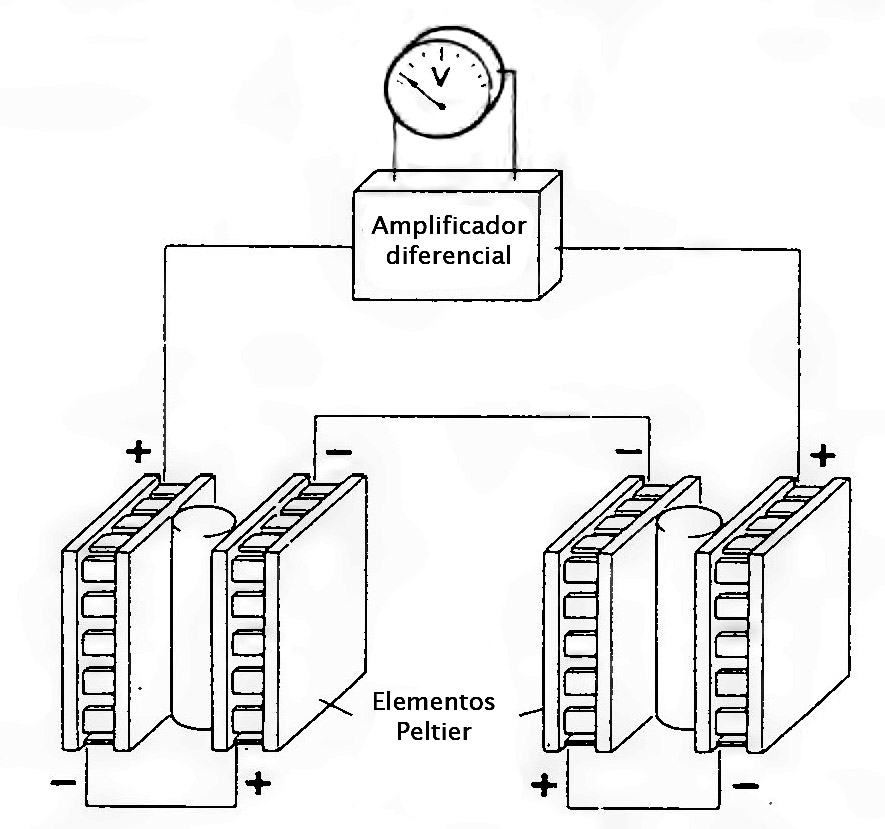
\includegraphics[width=\linewidth]{Figures/twinMeasuring}
			\caption{Principio de medici\'on de dos celdas gemelas, modificado de \cite{Suurkuusk}.}
			\label{fig: twin}
		\end{subfigure}
		\caption{Principio de detecci\'on de la energ\'ia transferida en forma de calor para cada canal de medida del calor\'imetro.}
	\end{figure}
	\newpage

	El calor\'imetro est\'a dise\~nado para que sea posible usar hasta cuatro cilindros de medici\'on independientes. Para cada uno de ellos, el principal camino del flujo de energ\'ia desde o hacia la celda es a trav\'es de los elementos Peltier \cite{Suurkuusk}. Dichos elementos est\'an compuestos de materiales semiconductores, sensibles a gradientes de temperatura del orden $1\times10^{-6}$ \grad{} \cite{Suurkuusk, simon2013oxford}. La uni\'on de estos semiconductores en serie, da lugar a detectores altamente sensibles a flujos de energ\'ia en forma de calor. Para detectar estos flujos se usa el efecto Seebeck, seg\'un el cual, para un gradiente de temperatura se genera una diferencia de potencial entre dos terminales de la celda. El efecto contrario recibe el nombre de efecto Peltier y se debe a que al pasar una corriente el\'ectrica a trav\'es de un material, se genera un transporte de energ\'ia en forma de calor. El flujo de energ\'ia t\'ermica se escribe de la siguiente forma \cite{simon2013oxford}:
	\begin{equation}\label{eq: peltier}
		\mathbf{j}^q = \Pi \mathbf{j}
	\end{equation}
	
	donde $\Pi$ recibe el nombre de coeficiente Peltier, $\mathbf{j}^q$ es la densidad de flujo de energ\'ia en forma de calor y $\mathbf{j}$ la densidad de corriente el\'ectrica \cite{simon2013oxford}. El coeficiente Seebeck ($S$) se define como $S = -\Delta V/\Delta T$ con $\Delta V$ como la diferencia de voltaje y se relaciona con el coeficiente de Peltier como: $\Pi = ST$, por lo cual al aplicar sobre la \autoref{eq: peltier} se obtiene:
	\begin{equation}\label{eq: seebeck}
		\mathbf{j}^q = (ST) \mathbf{j} = \left(-T\dfrac{\mathbf{j}}{\Delta T}\right)\Delta V = k\Delta V
	\end{equation}
	
	De esta forma se tiene que $\mathbf{j}^q \propto \Delta V$, por lo cual es posible cuantificar un flujo de energ\'ia t\'ermica en forma de calor con una lectura de potencial el\'ectrico. Las calibraciones el\'ectricas permiten determinar el valor de $k$, el cual, como se observa en la \autoref{eq: seebeck}, depende de la temperatura, por lo cual si se modifica la temperatura del ba\~no interno resulta necesario realizar una nueva calibraci\'on el\'ectrica. Dada esta dependencia con la temperatura, el calor\'imetro cuenta con un ba\~no termostatado con capacidad para 25 litros de agua, los cuales rodean los cilindros de medici\'on y act\'ua como reservorio t\'ermico \cite{Suurkuusk}. La sensibilidad a la temperatura hace que las funciones principales del calor\'imetro se encuentren divididas en dos unidades independientes, la del control de las condiciones isot\'ermicas y la detecci\'on de los eventos calorim\'etricos. La primera se encuentra descrita en el \autoref{ch: thermal}. Respecto a la segunda, la detecci\'on de los flujos de energ\'ia en forma de calor, el calor\'imetro usa dos celdas de medici\'on para cada canal de medida. Los elementos Peltier de cada canal se encuentran conectados en serie, pero con la polarizaci\'on opuesta, de tal forma que se registre la diferencia en los flujos de calor de las dos celdas, de esta forma es posible usar una para el estudio de la muestra (lado \texttt{A}) y otra para realizar un blanco (lado \texttt{B}) como se muestra en la \autoref{fig: twin}.
	 
	El calor\'imetro puede tomar medidas de celdas, las cuales pueden ser usadas para estudiar el crecimiento de microorganismos, o en modo de titulaci\'on, para el cual es necesario contar con un agitador permanente en la soluci\'on, as\'i como de un sistema de inyecci\'on para adicionar la soluci\'on titulante \cite{Suurkuusk}. Un ejemplo de esta aplicaci\'on es la calibraci\'on qu\'imica que se muestra en el \autoref{ch: chemical}, de donde se pueden obtener propiedades termodin\'amicas del sistema a partir de la potencia registrada este. 	 

\section{Justificación del proyecto}
	En general, la calorimetría permite una gran variedad de análisis, muchos de ellos cuentan con aplicaciones industriales, comerciales, biológicos y químicos, permitiendo el entendimiento de las interacciones moleculares en soluciones \cite{blandamer1998titration}. Una ventaja de la calorimetría es que no es específica, ni invasiva, además de no depender de las propiedades electroquímicas y ópticas de un sistema dado, siendo esto de vital importancia para las investigaciones de procesos biológicos, el estudio del crecimiento bacteriano y para la detección de compuestos biológicos \cite{winkelmann2004application}. Por otro lado la calorimetría también permite el estudio de la termodinámica en sistemas de adsorción, bien sea por la universalidad de la adsorción física en superficies como catalizadores, o en procesos industriales como la separación de mezclas de gases \cite{morrison1987calorimetry}. Finalmente la calorimetría es el método clásico para la determinación de propiedades termodinámicas en las muestras, entre estas se encuentran: capacidad calorífica, entalpía, entropía y energía libre de Gibbs, las cuales constituyen el punto de partida de gran cantidad de estudios teóricos, desarrollos y producción industrial de un compuesto químico \cite{wang2005determination, gaisford2016principles}.
	
	El calorímetro 2277 Thermal Activity Monitor con el que cuenta el grupo de investigación, al momento de realizar este trabajo se encontraba desarmado, a la espera de su instalaci\'on y puesta en funcionamiento. Este instrumento permite monitorear una gran variedad de reacciones químicas y bioquímicas, lo anterior debido a su capacidad de cuantificar procesos exotérmicos y endotérmicos. Estas reacciones pueden ser estudiadas en el rango de 5 - 80 $^\circ$C \cite{Suurkuusk}. Este rango de temperaturas se debe al uso de un baño termostatado de 25 litros. Cuatro balones de medición independientes se encuentran sumergidos en este baño, permitiendo medidas en el rango de microvatios \cite{Suurkuusk}. Es por esta razón que poner en marcha y calibrar el equipo con el que cuenta el grupo de investigación resulta una contribución importante para el mismo, así como para el \deptname.
	
\section{Objetivos}
	\subsection{Objetivo general}
		Poner en funcionamiento el calorímetro 2277 Thermal Activity Monitor con el que se cuenta, y adicionalmente calibrar el equipo para su uso en las investigaciones activas del grupo \groupname.
		
	\subsection{Objetivos específicos}
		\begin{itemize}
			\item Realizar el cableado y conexiones electrónicas pertinentes a la instalaci\'on del equipo 2277 Thermal Activity Monitor.
			\item Mantener la temperatura del ba\~no interno estable a una temperatura de 25 \grad{}.
			\item Realizar calibraciones eléctricas, para asegurar que las señales obtenidas tengan un equivalente en potencia.
			\item Determinación de la entalpía molar, energía libre de Gibbs, entropía, y constante de afinidad, de la reacci\'on de bicarbonato de potasio con \'acido clorh\'idrico como una calibración química.
		\end{itemize}